\documentclass[ms,thesis,twoside]{iist}

%% ---- Packages of use ---- %%

\usepackage[pdftex]{graphicx}
\usepackage[backend=biber, citestyle=authoryear, style=authoryear]{biblatex}
\usepackage{booktabs}
\usepackage{colortbl}
\usepackage{csquotes}
\usepackage{float}
\usepackage{layouts}
\usepackage{pdflscape}
\usepackage{subcaption}
\usepackage[normalem]{ulem}

%% ---- Figure Management ---- %%

\graphicspath{{./figures/}}

%% ---- Bibliography Management ---- %%

\addbibresource{doct.bib}

\title{Multimessenger constraints on outflows from neutron star mergers}
\author{B.S.Bharath Saiguhan}
\studentid{SC16B123}
\advisor{Dr. Resmi Lekshmi}
\specialization{Astronomy and Astrophysics}
\department{Earth and Space Sciences}
\date{\today}


%% ---- Document starts here ---- %%
\begin{document}

    \raggedbottom

    %% ---- Make the initial set of pages ---- %%

    \maketitle % Title page
    \makecertificate % Certificate
    \makedeclaration % Declaration
    \makededication % Dedication -- TODO
    \makeacknowledgements % Acknowledgements -- TODO
    \makeabstract % Abstract -- TODO
    \maketableofcontents % Table of contents -- TODO
    \makelistoffigures % List of figures -- TODO
    \makelistoftables % List of tables -- TODO
    \makelistofalgorithms % List of algorithms -- TODO
    \makeabbreviations % List of abbreviations -- TODO
    \makenomenclature % Nomenclature (for symbols used) -- TODO

    % Initialize chapter settings; DO NOT comment this line

    \makechaptersettings

    %% ---- Start chapters here ---- %%

    \chapter{Introduction}\label{ch:introduction}

\section{Outflows from BNS Mergers}
    \label{sec:bns}
    Due to the joint electromagnetic and gravitational wave detection of the
    binary neutron star coalescence known as GW1701817 (see
    \cite{abbott_gw170817_2017}), there has been renewed interest in sGRBs.
    Specifically, the claim that SGRBs have binary neutron star mergers as
    their central engines  (see \cite{narayan_gamma-ray_1992}) gained
    credence because of this detection. There are other aspects of the
    process that are not as clear. Specifically, several aspects of GW170817
    have not been completely explained. The main concerns are as follows
    \cite{lazzati_short_2020}:

    \begin{itemize}

        \item The outflow of GRB170817A was lower in energy, compared to that of
            a typical cosmological SGRB, by a factor of $10^4 - 10^5$, even
            though the event was one of the closest GW events recorded, at a
            distance of $\sim$ 40 Mpc. This could be due to two factors :

            \begin{itemize}

                \item The observer being off-axis with respect to the structured
                    jet.

                \item The internal engine powering this SGRB was intrinsically
                    less energetic, and differs from the one observed in other
                    typical SGRBs.
            \end{itemize}

        \item A clear consensus has not been reached on how the gamma-ray prompt
            emission was produced. The uncertainty partly comes from the fact
            that the various delays involved before the prompt emission is
            observed are not accurately constrained. Models which have been
            considered include :

            \begin{itemize}

                \item The structured outflow model, characterised by functions
                    for the Lorentz factor and the energy per unit solid angle,
                    both of which vary with the angle made with the polar jet
                    axis ($\theta$). This model produces detectable signals even
                    at moderately large off-axis angles.

                \item The shock breakout model, wherein the leading edge of the
                    wind emits the prompt emission as it breaks out of the
                    cocoon of nuclear matter ejected before the jet was
                    launched. This model has been shown to explain the
                    energetics and spectrum of the prompt emission, although it
                    does require a setup in which the wind is fast enough so
                    that it can reach a large enough distance at breakout.

            \end{itemize}

    \end{itemize}

    More light can be shed on these questions by observing more such SGRBs,
    using both the gravitational wave (GW) and electromagnetic (EM) windows.
    However, the possibility of joint detections are slim, due to the fact that
    the EM observations are highly dependent on the viewing angle of the system
    with respect to the observer (due to relativistic beaming), whereas GW
    signal amplitudes depend on the distance to the event
    \cite{saleem_prospects_2020}.\\ Given that this is the case, it is expedient
    to look for constraints on the structure parameters of various models.
    Furthermore, it is useful to develop models which are resilient to
    non-detections, and can produce constraints on the parameters using upper
    limits on the flux/fluence observed by the various EM follow-up satellites,
    such as INTEGRAL, Fermi or Swift.

    As mentioned before, the electromagnetic follow-up of the binary neutron
    star merger event GW170817 helped measure the various time delays between
    the time of the GW signal trigger (which roughly is the merger time itself)
    and the time the gamma-ray signals were picked up. This time delay is
    denoted $\Delta t_{GW-\gamma}$, and was around 1.75 seconds for this event.
    The components which make up this delay are as follows
    \cite{lazzati_short_2020}:

    \begin{itemize}

        \item \textbf{Engine Delay} : this is the delay due to some transition
            mechanism in the central engine which powers the jet (such as a
            metastable, fast spinning neutron star which collapses into a black
            hole when its rotation period increases; this process can take
            years) or due to the need of amplifying the magnetic field to a
            value large enough to launch the jet  (this process is significantly
            faster, taking seconds). This is denoted by $\Delta t_{eng}$.

        \item \textbf{Wind Delay} : this is simply a delay in the launching of a
            non-relativistic wind due to the neutron-rich matter from the
            progenitors being tidally shredded. For this reason, it can be
            \textit{negative} as well, since the tidal shredding can occur
            before the merger itself. This is denoted as $\Delta t_{wind}$.

        \item \textbf{Breakout Delay} : if the wind is ejected before the jet,
            then the latter will have to propagate through the former and this
            happens at a sub-relativistic speed, whereas the GW signal travels
            at a relativistic speed. The delay due to this crossing is the
            breakout delay, and is denoted $\Delta t_{bo}$. During this time,
            jet-wind interactions cause the development of a structured outflow
            that maintains a bright core but also has energetic wings at large
            polar angles.

        \item \textbf{Photospheric Delay} :  once the jet has crossed the wind,
            it still needs to propagate out to the photospheric radius, where
            the outflow becomes transparent and the prompt gamma-ray emission is
            radiated. The delay from the breakout radius to the photospheric
            radius is $\Delta t_{ph}$. This is given as (for GW170817):

            \begin{equation}
                \label{eq:4}
                \Delta t_{ph} \sim \dfrac{R_{ph}}{c \Gamma^2} =
                1.4 \dfrac{R_{ph}}{2 \times 10^{12} \text{ cm}}
                \left( \dfrac{7} {\Gamma} \right)^2 \text{ s}
            \end{equation}

        \item \textbf{Dissipation Delay} : this is a requirement in some models,
            such as the internal shock synchrotron model, wherein the outflow
            needs to travel to the internal shock radius before the bulk energy
            of the flow is dissipated and turned into radiation. The time
            required to get to this point after crossing the photospheric radius
            is the dissipation delay, denoted $\Delta t_{\gamma}$

    \end{itemize}


    Several attempts to constrain the various time delay components have been
    made. However, except for relative comparisons, no conclusions have been
    arrived upon.  For example, one can only say that the photospheric delay is
    the major component out of all the delays, and that wind delay (if non-zero)
    has to be lesser than the jet delay, so that the jet catches up to the wind
    and the jet-wind interaction generates the structured outflow. The figure
    below summarises these delays in the broader context.

    \begin{figure}[H]
        \label{fig:jet_delay}
        \centering
        \includegraphics[width=12cm]{jet_delay}
        \caption[Relative Positions of Jet Delays]{
                    Two possible scenarios for the relative positioning of the
                    delays in time, which contribute to $\Delta t_{GW-\gamma}$.
                    Owing to the requirement of a structure outflow, GW170817
                    possibly follows the top timeline. The relative
                    contributions of the various delays are debated, but it is
                    agreed that $\Delta t_{wind} < \Delta t_{jet} \ll 1$ s,
                    $\Delta t_{bo} \ll 1$ s, $\Delta t_{\gamma} \sim 0$ and
                    $\Delta t_{ph} \sim \Delta t_{GW-\gamma}$.
             }
    \end{figure}

    Due to the uncertainties in the delay terms, several models for the jet can
    explain the energetics and observed structure. Numerical simulations are
    also not unequivocal about their favouring of one model over the other (see
    \cite{shibata_merger_2019}). Some models try to explain the apparent
    structure of the jet, that is the observables seen by a particular observer
    at a particular viewing angle. Other models are used to explain the
    \textit{intrinsic} structure, such as the polar angle variation of the bulk
    Lorentz factor and the energy across the solid angle, in the jet co-moving
    frame (see \cite{salafia_structure_2015} for a detailed discussion of the
    differences between the two structures). Some of these are given below (see
    also Figs. \ref{fig:tophat} and \ref{fig:jet_models}):

    \begin{itemize}

        \item Top-hat : This model, as used in \cite{saleem_energetics_2020},
            assumes that the bulk Lorentz and energy functions drop to zero
            beyond some cutoff angle, $\theta_j$. Below this threshold, the
            functions are at their respective on-axis values.

       \item Gaussian : This model is widely used, in some contexts to explain
           the apparent jet structure (by \cite{hayes_comparing_2020}), and in
           others the intrinsic jet structure (by
           \cite{saleem_energetics_2020}). The former is simply given by
           $y_{GJ}(\theta) = e^{- \frac{1}{2} \left(
           \frac{\theta}{\theta_{\sigma}} \right)^2}$, since the authors
           consider only the apparent jet structure, as explained above and
           $\theta_\sigma$ is a structure parameter which is inferred by the
           authors' Bayesian inference.\\
           In the latter, as the authors consider the intrinsic jet structure,
           they assume that $\Gamma \beta (\theta)
           = \Gamma_0 \beta_0 \exp\left(- \theta^2 / 2\theta_c^2\right)$ and
           that $\epsilon (\theta) \propto \exp(- \theta^2 /
           \theta_c^2)$\footnote{This is the normalised energy profile function.
           The normalisation constant is estimated by the condition $2\pi \int
           d(\cos \theta) \epsilon(\theta) = E_{tot., \gamma}$, where $E_{tot.,
           \gamma}$ is the total energy in gamma-rays.}, and derive the observed
           properties (see below).

        \item Power Law : This model is used by \cite{hayes_comparing_2020} to
            explain the apparent structure of the jet, assuming that any
            variation in the energy is simply because of relativistic beaming
            and the jet being viewed off-axis. It is given using the shape
            function $y(\theta)$ (which is multiplied with the on-axis isotropic
            equivalent energy $E_{iso, 0}$ to give
            $E_{iso}(\theta)$\footnote{Using the equation $E_{iso}(\theta_v) =
            E_{iso, 0} \cdot y(\theta_v)$}):

                \begin{equation}
                    \label{eq:5}
                    y(\theta) = \begin{cases}
                                    1,
                                        & 0 \leq \theta \leq \theta_c, \\
                                    (\theta/\theta_c)^{-2},
                                        & \theta_c < \theta \leq \theta, \\
                                    0,
                                        & \theta_j < \theta
                                \end{cases}
                \end{equation}
                Here $\theta_c$ and $\theta_j$ are simply structure parameters,
                inferred using Bayesian methods.

    \end{itemize}

    \begin{figure}[H]
        \centering
        \includegraphics[width=9cm]{tophat}
        \caption[Tophat jet structure model]{
                    Functional form of the tophat jet structure model, as considered in
                    \cite{saleem_energetics_2020}. The dashed line denotes the jet angle
                    $\theta_j = 15^{\circ}$.
             }
        \label{fig:tophat}
    \end{figure}

    \begin{figure}[H]
        \centering
        \includegraphics[width=\textwidth]{jet_models}
        \caption[Jet structures as in \cite{hayes_comparing_2020}]{
                    Functional forms of the jet structure models, as considered by
                    \cite{hayes_comparing_2020}. (Left) The gaussian jet structure with
                    a width $\theta_{\sigma} = 20^{\circ}$, also marked by the dashed
                    line. (Right) The power-law structure with a core angle $\theta_c =
                    8^\circ$ and a jet angle $\theta_j = 32^\circ$.
             }
        \label{fig:jet_models}
    \end{figure}

    In order to start off with an intrinsic structure and calculate the observed
    structure, following \cite{granot_off-axis_2002}, we start off by
    considering the emission profile of a point source moving at some angle with
    the observer, essentially rendering this scenario off-axis. This will affect
    the prompt jet emission, as well as the initial afterglow, and so warrants
    careful analysis.  Now, let the initial jet opening angle be $\theta_0$ and
    let the observer be at an angle $\theta_{obs}$. In general, for a point
    source moving at any angle $\theta$ with respect to the observer, the
    observed flux is given by :

    \begin{equation}
        \label{eq:1}
        F_{\nu} =
           \dfrac{L^{\prime}_{\nu^{\prime}}}{4 \pi d_L^2}
           \left( \dfrac{\nu}{\nu^\prime}\right)^3
                =
            \dfrac{1 + z}{4 \pi d_L^2}
            \dfrac{L^{\prime}_{\nu^{\prime}}}{\gamma^3 (1 - \beta \cos \theta)^3}
    \end{equation}

    Here, $L^{\prime}_{\nu^{\prime}}$ and $\nu^{\prime}$ are the jet comoving
    frame spectral luminosity and frequency, $d_L$ is the luminosity distance,
    $\gamma = (1 - \beta^2)^{-1/2}$ is the jet Lorentz factor. If $t$ and $\nu$
    are the observed time and frequency  for an observer at $\theta$, and $t_0$
    and $\nu_0$ are those for an observer on the axis, then:

    \begin{equation}
        \label{eq:2}
        \dfrac{t_0}{t} =
            \dfrac{\nu}{\nu_0}
                       =
            \dfrac{(1 - \beta)}{(1 - \beta \cos \theta)}
            \equiv a
            \approx \dfrac{1}{(1 + \gamma^2 \theta^2)}
    \end{equation}

    And finally putting Eq. \ref{eq:2} into Eq. \ref{eq:1} and expanding using a
    Taylor series approximation upto the leading order:

    \begin{equation}
        \label{eq:3}
        F_{\nu}(\theta_{obs}, t) =
            a^3
            F_{\nu/a}(0, at)
    \end{equation}

    This gives us a handle on how to relate observed off-axis quantities to the
    on-axis ones. Furthermore, this enables us to go from an intrinsic structure
    to an observed one, which is what was required.

\section{Outflows from NSBH Mergers}

    The difference in this pathway to sGRBs, compared to the case of BNS mergers, is
    that though there is theoretical and simulational support for the launching of sGRB
    jets from the merger of a neutron star and a black hole of appropriate mass (see for
    example \textbf{citations}), there has not been strong evidence from the
    observational side of things. In the first half of the third observing run of the
    LVC (also known as O3a), there have been several triggers which have been reportedly
    confident NSBH triggers. However, there were no counterpart EM signals picked up,
    which decreases the credibility of NSBH mergers as the progenitors of sGRBs.\\

    The electromagnetic component from NSBH mergers, is largely decided based on the
    amount of mass left post-merger, outside the horizon of the black hole. This decides
    how much matter participates in the subsequent processes, which may be the rapid
    neutron-capture process which gives rise to the kilonova signal or the magnetic
    field amplification via magneto-rotational instability which leads to a sGRB jet.\\

    Qualitatively, for a binary where the neutron star is treated as a test mass and the
    black hole's spin is aligned with the orbital angular momentum of the binary, the
    innermost-stable circular orbit radius $r_{ISCO}$ scales as $r_{ISCO} \sim
    f(\chi_{BH}) G M_{BH}/c^2$ (where f is a function ranging from 1 to 9, decreasing
    for increasing (prograde) spins; see \cite{bardeen_1972}) and the radius at which
    the tidal disruption of the neutron star starts, $r_{dis}$ scales as $r_{dis} \sim k
    (M_{BH/M_{BNS}})^{1/3} R_{NS}$ (where k is a constant with a dependence on the black
    hole spin and the equation of state). Only requiring that $r_{dis} \gtrsim
    r_{ISCO}$, as a rough requirement for disruption to occur before the neutron star
    plunges into the black hole, leads to the conclusion that (a.) low-mass black holes
    (b.) larger NS radii (c.) higher prograde black hole spins favour disruption. This
    is seen as well from Fig. \ref{fig:nsbh_disruption_condition}. However, the actual
    quantitative results need to be simulated such the effect of the various components
    in the problem are correctly taken into account. As seen from carrying these
    simulations out, the matter left over post-merger heavily depends on (for a summary,
    see Fig. \ref{fig:rest_mass_fraction}):

    \begin{itemize}

        \item The mass ratio of the system. This is defined as $q = M_{BH} / M_{NS}$ so
            that $q > 1$ always. Fully general relativistic, magnetohydrodynamic
            simulations (such as \cite{ruiz_2020}) show that in cases where the  mass
            ratio is 3:1, regardless of the neutron spin, a collimated outflow is
            observed, whereas the same is not realised in cases where the mass ratio is
            5:1 or higher.
        \item The spin of the components of the system. In geometrized units (where $G =
            c = 1$), these are prescribed in terms of $a_{BH} / M_{BH}$ or $a_{NS} /
            M_{NS}$, and whether these two spins align (prograde) or are anti-aligned
            (retrograde) decides whether the neutron star would be tidally disrupted,
            and hence participate in the processes mentioned previously, or not. Via
            simulations, it is seen that the more the prograde spin of the neutron star,
            the farther out the neutron star is tidally disrupted, albeit this is only
            observed for the case of q = 3:1 (comparing say, Figs. \ref{fig:nsbh_jet}
            and \ref{fig:nsbh_5to1}). Also, this leads to long tidal tails, which
            produces a baryon-loaded environment and thus the magnetic field of the
            tidally disrupted matter must overcome the baryon ram pressure to launch the
            jet. This process hence delays the launching of the jet.
    \end{itemize}

    Aside from the sGRB jet, which requires magnetic field amplification (via MRI) as
    well as thermal pair production (from the disk remnant) followed by the
    Blandford-Znajek process, there is a possibility that NSBH mergers can produce
    kilonovae signatures. For this, the dynamically ejected mass has to be between
    $10^{-4.5} - 10^{-2} (M_{NS}/1.4 M_{\odot}) M_{\odot}$ (see \cite{ruiz_2020} for
    more details), and this will lead to kilonovae potentially detectable by the Large
    Synoptic Survey Telescope (LSST).

    \begin{figure}[H]
        \centering
        \includegraphics[width=\textwidth]{nsbh_jet}
        \caption[Tidal disruption of a NS in a 3:1 NSBH binary]{
                    Volume rendering of the rest mass density ($\rho_0$) (in log scale),
                    normalized to the NS maximum value $\rho_0 = 8.92 \times 10^{14}
                    (1.4 M_{\odot}/M_{NS})^2 \text{ g/cm}^3$, for particular times for a
                    magnetized neutron star, with q = 3:1 and a prograde NS spin of
                    0.23.  Top three panels highlight the inspiral and the tidal
                    disruption, whereas the bottom three panels highlight the appearance
                    of the magnetically-driven jet. White lines denote the magnetic
                    field, arrows denote the fluid velocity and the BH's apparent
                    horizon is the black sphere. Here M = $2.5 \times 10^{-2}
                    (M_{NS}/M_{1.4M_{\odot}}) \text{ ms} = 7.58
                    (M_{NS}/M_{1.4M_{\odot}}) \text{ km}$ (in geometrized units). From
                    \cite{ruiz_2020}.
             }
        \label{fig:nsbh_jet}
    \end{figure}

    \begin{figure}[H]
        \centering
        \includegraphics[width=\textwidth]{nsbh_5to1}
        \caption[Tidal disruption of a NS in a 5:1 NSBH binary]{
                    Similar to Fig. \ref{fig:nsbh_jet}, however with the NS spin being
                    0.33, the BH spin being 0 and q = 5:1. In this case, no strong
                    collimation of the magnetic field is observed from the merger
                    remnant, and so a magnetically-driven jet is also not observed.
                    From \cite{ruiz_2020}.
            }
        \label{fig:nsbh_5to1}
    \end{figure}

    \begin{figure}[H]
        \centering
        \includegraphics[width=11cm]{rest_mass_fraction}
        \caption[Rest mass outside black hole horizon, as a function of time]{
                    Fraction of rest-mass of the NS outside the apparent horizon of the
                    black hole as a function of coordinate time, for the various
                    configurations considered in \cite{ruiz_2020}. The inset figures
                    report the same for non-magnetized cases, and the coordinate time is
                    shifted such that the merger time coincides with 0.
            }
        \label{fig:rest_mass_fraction}
    \end{figure}

    \begin{figure}[H]
        \centering
        \includegraphics[width=11cm]{nsbh_disruption_condition}
        \caption[Disruption condition in a NSBH binary]{
                    Maximum value of the mass-ratio ($M_{BH}/M_{NS}$) for which a NSBH system
                    disrupts, as a function of the neutron star radius $R_{NS}$, and the aligned
                    component of the dimensionless black hole spin $\chi_{BH}$, assuming $M_{NS} =
                    1.35 M_{\odot}$. Results for other neutron star masses can be obtained by
                    rescaling considering the disruption condition at constant compaction $C_{NS} =
                    GM_{NS}/R_{NS} c^2$. From \cite{foucart_2020}.
            }
        \label{fig:nsbh_disruption_condition}
    \end{figure}
  % Introduction
                      % TODO: Fix to make appropriate

    \chapter{Population Synthesis}\label{ch:synthesis}
    In order to derive meaningful conclusions about the outflows from NS mergers, given
    the models described in \ref{ch:introduction}, it was necessary to carry out
    population synthesis studies. In these, population models which are physically or
    observationally motivated are taken from the literature and used to compute the
    statistical properties of the outflows from NS mergers created with these
    properties. If no confident or relevant model exists in literature, physically
    motivated ans\"{a}tze are used (see for example, \S\S\ref{sub:spin-dists}).\\
    In each study which uses (slightly) different population models, 10$^5$ samples were
    drawn from the relevant parameter distributions. Using these as inputs the expected
    outflows were calculated using the fit formulae described in
    \ref{ch:introduction}.\\
    In this chapter, the various population models are briefly described along with
    their pertinence. Furthermore, preliminary checks for the population synthesis code
    are also discussed, which help verify the consistency of the code with theoretical
    results.

\section{Black Hole Population Models}\label{sec:bh_pop}

    \subsection{Mass, $M_{BH}$}
        The masses of the black holes was sampled from the `truncated' mass distribution
        from \cite{abbott_2020B}. The distribution `produces' black holes with masses
        between 3--100 M$_\odot$ (as can be seen from Fig.  \ref{fig:bh_mass_gwtc2}).
        However, NS binaries with extremely massive ($M_{BH} > 20 M_\odot$) black holes
        will not produce any appreciable EM emission due to the NS companion plunging
        into the black hole directly without significant tidal disruption. For this
        reason the population synthesis code imposes an upper limit to the black hole
        masses sampled.

        \begin{figure}[H]
            \centering
            \includegraphics[width=\linewidth]{bh_mass_gwtc2}
            \caption[Black hole mass distributions from GWTC-2]{
                Black Hole Mass Distributions from \cite{abbott_2020B}. In the current
                study the `truncated' mass distribution with an upper limit at 20
                M$_\odot$, since more massive black holes would not produce significant
                EM emission when in a merging NSBH binary.
            }
            \label{fig:bh_mass_gwtc2}
        \end{figure}

        \begin{figure}[H]
            \centering
            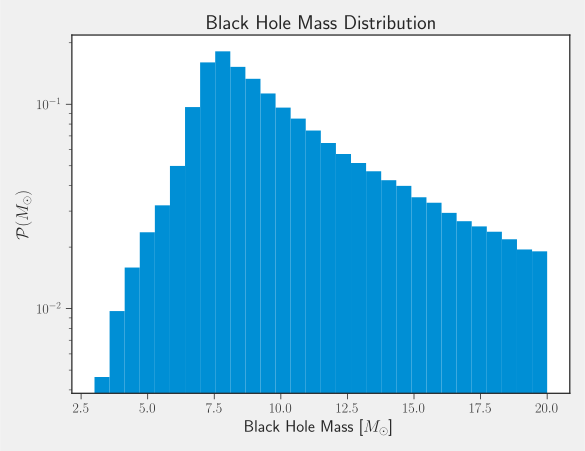
\includegraphics[width=0.8\linewidth]{bh_mass}
            \caption[Black hole mass distribution with upper limit]{
                Black hole mass distribution as used in the current report, with an
                upper limit of 20 M$_\odot$.
            }
            \label{fig:bh_mass}
        \end{figure}

    \subsection{Spin, $chi_{BH}$}\label{sub:spin-dists}
        The spins of the black holes are sampled from the `default' distribution given
        in \cite{abbott_2020B}. This distribution is essentially a Beta distribution
        , which ensures that the spin parameters sampled from this distribution remain
        within [0, 1).\\

        \begin{figure}[H]
            \centering
            \includegraphics[width=0.8\linewidth]{bh_spin_gwtc2}
            \caption[Black hole spin distribution from GWTC-2]{
                Beta distribution for the  black hole spin from \cite{abbott_2020B}.
                Here the light traces are samples from the posterior distribution,
                whereas the solid black line is the posterior probability distribution
                for $\chi_{BH}$. Dashed black lines mark the 90\% quantiles for the
                same.
            }
            \label{fig:bh_spin_gwtc2}
        \end{figure}

        However, since there have been no confident NSBH merger detections in the GW
        regime, this distribution is largely derived from looking at BBH mergers, and so
        may not represent the true spin distribution of a black hole in a NSBH binary.
        To circumvent this, the following ans\"{a}tze are used to probe the effect of
        the spin distribution on the EM outflows:

        \begin{itemize}

            \item Uniform spin distribution: here $\chi_{BH} \sim \mathcal{U}(0, 1)$.
                Note also that this distribution will have a higher number of high spin
                samples as compared to the `default' distribution considered above.

            \item Gaussian spin distribution: here $\chi_{BH} \sim \mathcal{N}(\mu,
                \sigma)$, but samples outside of [0, 1) are not considered. For
                simplicity and to cover a representative sample of the possible
                distributions, samples were taken from $\mathcal{N}(0.2, 0.2)$,
                $\mathcal{N}(0.5, 0.2)$ and $\mathcal{N}(0.7, 0.2)$. These represent
                distributions concentrated around low, medium and high spins
                respectively.

        \end{itemize}

        % TODO: insert figures for the uniform and gaussian spin distributions!

\section{Neutron Star Population Models}\label{sec:ns_pop}

    In order to reduce the number of variables in the problem, the masses of all neutron
    stars in the population was set to 1.4 M$_\odot$. This value corresponds to the
    median neutron star mass as inferred from GW170817 (see \cite{abbott_2018}). Also,
    the spins of all neutron stars was set to 0, since it is assumed that sufficient
    amount of time would have passed between the formation of the binary and merger,
    allowing for the neutron star to spin down such that $\chi_{NS} \sim 0$.\\
    Additionally, the tidal deformability of the neutron stars was set using the C-love
    relation (see \cite{yagi_2017}). First, the radii of the neutron stars were set to
    11 km, which is the median neutron star radius inferred for GW170817. Then, the
    compactness of the neutron stars, $C_{NS}$ was computed using the relation :

    \begin{equation}
        C_{NS} = \dfrac{G M_{NS}}{R_{NS} c^2}
    \end{equation}

    where $M_{NS}$, $R_{NS}$ are the mass and radius of the neutron star, G is the
    universal gravitational constant and c is the speed of light.  Finally, the tidal
    deformability is computed by solving the C-Love relation :

    \begin{equation}
        C_{NS} = \sum_{k=0}^{2} a_k (\ln \Lambda_{NS})^k
    \end{equation}

    where $\Lambda_{NS}$ is the tidal deformability of the neutron star, and $a_k$ are
    the fit coefficients as given in \cite{yagi_2017}.

\section{Spatial Distribution and Orientation of events}\label{sec:space_dist}

    \subsection{Constant comoving volume distribution}

        The events whose component mass and spin distributions were described in
        \ref{sec:bh_pop}-\ref{sec:ns_pop} are distributed in 3D space such that their
        number density is constant in comoving volume.\\
        For this, firstly the latitudinal ($\theta$) and longitudinal ($\phi$) angles
        are sampled such that $\cos \theta \sim \mathcal{U}(-1, 1)$ and $\phi \in
        \mathcal{U}(0, 2\pi)$, i.e. they are sampled such that they are uniform on a
        unit sphere. As for the comoving distance distribution $\mathcal{P}(D_c)$,
        consider the probability of an event lying in an infinitesimal shell of width
        d$D_c$ at a comoving distance $D_c$.  Then it can be seen that:
        \begin{equation}
            \mathcal{P}(D_c) dD_c \propto D_c^2 dD_c \Rightarrow
                \boxed{\mathcal{P}(D_c) = \alpha D_c^2}
        \end{equation}
        where $\alpha$ is the constant of proportionality. In the local universe, it can
        be safely assumed that $D_c \approx D_L$, where the latter is the luminosity
        distance.  However, from the fact that the GW SNR $\rho \propto D_L^{-1}$ it can
        also be seen that:

        \begin{align}
            \mathcal{P}(\rho) &= \mathcal{P}(D_L)
                                  \Big \lvert \dfrac{dD_L}{d\rho} \Big \rvert \\
                              &= \mathcal{P}{D_c}
                                  \Big \lvert \dfrac{dD_c}{d\rho} \Big \rvert \\
                              &\propto \dfrac{1}{\rho^2} \dfrac{1}{\rho^2}
                                  = \dfrac{1}{\rho^4} \nonumber\\
            \Rightarrow \mathcal{P} (\rho) &= \dfrac{\beta}{\rho^4}
        \end{align}

        Once the SNR detection threshold\footnote{
            This is defined such that any event with a GW network SNR greater than the
            detection threshold will be considered a detection.
        } ($\rho_{th}$) is set, the normalization constants can be computed as follows:

        \begin{align}
            \int_0^{D_{c, max}}
                \mathcal{P}(D_c) dD_c &= \int_0^{D_{L, max}} \mathcal{P}(D_L) dD_L \\
                                      &= \int_0^{\rho_{th}} \mathcal{P}(\rho) d\rho \\
                                      &= 1
        \end{align}

        This gives:

        \begin{align}
            \label{eq:lum_dist}
            \mathcal{P}(D_L) = 3 \dfrac{D_L^2}{D_{L, max}}
                                 \Leftrightarrow
            \mathcal{P}(\rho) = 3 \dfrac{\rho_{th}^3}{\rho^4}
        \end{align}

        where $D_{L, max}$ is the luminosity distance corresponding to the detection
        threshold. As an example, for the Advanced LIGO/VIRGO configuration and a SNR
        threshold of 10, $D_{L, max} \approx 1123$ Mpc.\\
        Using Eq.\ref{eq:lum_dist}, samples are drawn from the luminosity distance
        distribution and using the previous samples for $\theta$ and $\phi$, events are
        distributed in 3D space such that the number density of events is constant in
        the comoving volume.

    \subsection{Orientation of Events}\label{sub:orientation_of_events}

        The orientation of NSBH binaries with respect to the line-of-sight is prescribed
        using the inclination angle, $\iota$ and the polarization angle of the incoming
        GW signal, $\psi$. These are distributed for the population such that $\cos\iota
        \sim \mathcal{U}(-1, 1)$ and $\psi \sim \mathcal{U}(0, 2\pi)$, from which
        samples are drawn for individual events.

\section{Summary}
  % About Popln Syn. Code
                      % TODO: add more info

    \chapter{Population Analysis}\label{chp:analysis}

\section{Summary}
  % Science from Population
                      % TODO

    \chapter{NS Merger Candidates in GWTC-2}\label{ch:candidates}

\section{About GWTC-2}

    The first half of the third observing run (O3a) of the LVC started on the 1st of
    April 2019, and went on till 30th of September, 2019.  Following this, instrumental
    upgrades were made during the month of October and the second half of the third
    observing run (O3b) was started on the 1st of November. Due to the global pandemic,
    the observing run had to be prematurely suspended on 30th of March, 2020.\\ Starting
    with O3, alerts were distributed via the public alerts section of Gravitational-wave
    Candidate Event Database (GRACE-DB). If triggers were registered that passed the
    detection threshold of the LVC network during observational runs, online parameter
    estimation was done using the raw GW data, and low latency estimates of the rough
    sky position, component masses and luminosity distance was made available for
    observers in the EM regime. This allowed for rapid follow-up in various bands of the
    electromagnetic spectrum, and these observations were reported and cross-verified
    using NASA's GRB Coordinates Network (GCN). Using the circulars reported in the GCN
    for NSBH/BNS events of interest, along with the low-latency information from
    GRACE-DB, O3a's non-BBH candidate events have been collected in table \ref{tab:gcns}
    \\ More detailed analysis of these events in the months following has led to at
    least 53 events in the third observing run alone. These can be classified as:
    \begin{itemize}

        \item 37 Binary Black Hole (BBH) merger candidates.

        \item 7 BNS merger candidates. Of these, only 1 corresponds to O3a, which is the
            event GW190425 discussed in the chapter \textbf{sec:190425}.

        \item 4 events in the mass gap, which are events with compact objects with
            masses of 3-5 $M_{\odot}$.

        \item 5 NSBH merger candidates. Of these, only 1 has been confirmed officially,
            which is the event GW190814.

    \end{itemize}

    Of these, 26 events were officially confirmed and 13 new events were reported for
    the first time in \cite{abbott_2020}, and it is from there that the posterior
    distributions of the various parameters (such as inclination angle $\iota$,
    luminosity distance $D_L$ etc) are used for further analysis.  Note also that there
    are several marginal events that have been reported, in that they have
    non-negligible probability distributed between two classifications. For example, the
    event GW190426\_152155 has significant probability split between it being a
    terrestrial event (58 \%) and a NSBH/BNS/Mass Gap event (cumulatively 42\%). Without
    a significant EM counterpart, this event cannot be confidently placed in either of
    the classes, and thus warrants further analysis. This is the subject of chapter
    \textbf{sec:190426}.

    \begin{table}[H]  % now this is how you format a table ;)
        \centering
        \setlength{\extrarowheight}{0pt}
        \addtolength{\extrarowheight}{\aboverulesep}
        \addtolength{\extrarowheight}{\belowrulesep}
        \setlength{\aboverulesep}{0pt}
        \setlength{\belowrulesep}{0pt}
        \begin{tabular}{cccccc}
            \toprule
            \rowcolor[rgb]{0.71,0.851,1}
            \begin{tabular}[c]{@{}>{\cellcolor[rgb]{0.71,0.851,1}}c@{}}
                \textbf{GRACE-DB} \\
                \textbf{Superevent} \\
                \textbf{ID}
            \end{tabular} &
            \textbf{$\mathcal{P}$(BBH)} & \textbf{$\mathcal{P}$(BNS)} &
            \textbf{$\mathcal{P}$(MassGap)} & \textbf{$\mathcal{P}$(NSBH)} &
            \textbf{$\mathcal{P}$(Terr)}  \\
            \hline \uline{S190426c} & 0 & 24 & 12 & 6 & 58\\
            S190910h & 0 & 61 & 0 & 0 & 39 \\
            S200213t & 0 & 63 & 0 & 0 & 37 \\
            S191213g & 0 & 77 & 0 & 0 & 23 \\
            S190901ap & 0 & 86 & 0 & 0 & 14 \\
            \uline{S190425z} & 0 & \textbf{\textgreater{}99} & 0 & 0 & 0 \\
            S190930s & 0 & 0 & 95 & 0 & 5 \\
            S190923y & 0 & 0 & 0 & 68 & 32 \\
            S190930t & 0 & 0 & 0 & 74 & 26 \\
            S191205ah & 0 & 0 & 0 & 93 & 7 \\
            S190910d & 0 & 0 & 0 & 98 & 2 \\
            S190814bv & 0 & 0 & 0 & \textbf{\textgreater{}99} & 0 \\
            \bottomrule
        \end{tabular}
        \caption[Candidate Merger Events and GRACE-DB Superevent IDs]{
                List of candidate merger events and the probability of
                classification (reported in \%) for each non-BBH event reported
                during O3a. Here the GRACE-DB superevent ID is used (instead of the
                GWTC-2 event ID), since for a particular GW event, the superevent
                collects both the EM followup as well as GW trigger information
                within GRACE-DB. The probabilities are assigned using the process
                described in \cite{kapadia_2020}, and are reported
                in GRACE-DB. The events underlined are discussed in more detail in
                later chapters.
            }
    \end{table}


    \begin{table}[H]
        \centering
        \setlength{\extrarowheight}{0pt}
        \addtolength{\extrarowheight}{\aboverulesep}
        \addtolength{\extrarowheight}{\belowrulesep}
        \setlength{\aboverulesep}{0pt}
        \setlength{\belowrulesep}{0pt}
        \begin{tabular}{cccc}
            \toprule
            \rowcolor[rgb]{0.71,0.851,1}
            \textbf{UID} & \textbf{FAR} & \textbf{$D_L$ (Mpc)} &
            \begin{tabular}[c]{@{}>{\cellcolor[rgb]{0.71,0.851,1}}c@{}}
                \textbf{Error in $D_L$} \\
                \textbf{(Mpc)}
            \end{tabular}  \\
            \hline
            \uline{S190426c} & 1 per 1.6276 yr & 377 & 100 \\
            S190910h & 1.1312 per yr & 230 & 88 \\
            S200213t & 1 per 1.7934 yr & 201 & 80 \\
            S191213g & 1.1197 per yr & 201 & 81 \\
            S190901ap & 1 per 4.5093 yr & 241 & 79 \\
            \uline{S190425z} & 1 per 69834 yr & 158 & 43 \\
            S190930s & 1 per 10.534 yr & 709 & 191 \\
            S190923y & 1.5094 per yr & 438 & 133 \\
            S190930t & 1 per 2.0536 yr & 108 & 38 \\
            S191205ah & 1 per 2.5383 years & 385 & 164 \\
            S190910d & 1 per 8.5248 years & 606 & 197 \\
            S190814bv & 1 per 1.559e+25 years & 241 & 26 \\
            \bottomrule
        \end{tabular}
        \caption[Candidate Merger Events and FARs]{
                List of candidate merger events and the probability of
                classification for each non-BBH event reported during O3a. FAR
                refers to the False Alarm Rate (in number of events per year or
                equivalently in Hz$^{-1}$), and $D_L$ is the luminosity distance.
                Both these values are those reported in GRACE-DB corresponding to
                each event. The events underlined are discussed in more detail in
                later chapters.
            }
    \end{table}

    \begin{table}[H]
        \centering
        \setlength{\extrarowheight}{0pt}
        \addtolength{\extrarowheight}{\aboverulesep}
        \addtolength{\extrarowheight}{\belowrulesep}
        \setlength{\aboverulesep}{0pt}
        \setlength{\belowrulesep}{0pt}
        \begin{tabular}{ccccc}
            \toprule
            \rowcolor[rgb]{0.71,0.851,1}
            \textbf{UID} &
            \textbf{FERMI-LAT} &
            \textbf{FERMI-GBM} &
            \textbf{SWIFT/BAT} &
            \textbf{INTEGRAL} \\
            \hline
            \uline{S190426c} & 24342 & 24248 & 24255 & 24242\\
            S190910h & 25742 & 25714 & 25718 & 25709 \\
            S200213t &
                27062 &
                {\cellcolor[rgb]{1,0.749,0.749}} \textcolor{red}{27056} &
                {\cellcolor[rgb]{1,0.749,0.749}} \textcolor{red}{27058} &
                27050 \\
            S191213g & 26412 & 26409 & 26410 & 26401 \\
            S190901ap & 25625 & 25610 & 25617 & 25605 \\
            \uline{S190425z} &
                24266 &
                24185 &
                24184, 24296 &
                \begin{tabular}{c}
                    24169, 24170 \\
                    24178, 24181
                \end{tabular} \\
            S190930s & 25895 & 25886 & 25889 & 25872 \\
            S190923y & 25834 & 25823 & 25846 & 25815, 25825 \\
            S190930t & 25898 & 25887 & 25888 & 25880 \\
            S191205ah & 26363 & 26359 & 26365 & 26531 \\
            S190910d & 25717 & 25699 & 25704 & 25698 \\
            S190814bv & 25385 & 25326 & 25341 & 25323 \\
            \bottomrule
        \end{tabular}
        \caption[Candidate merger events and relevant GCNs]
            {
                List of candidate merger events and the probability of
                classification for each non-BBH event reported during O3a. Here the
                GCN Circular number reporting the findings of the particular
                instrument in the column heading is reported, corresponding to each
                event. The events underlined are discussed in more detail in later
                chapters. GCNs marked with red should be ignored during analysis
                since they correspond to times when the respective instruments were
                in the South Atlantic Anomaly (SAA).
            }
        \label{tab:gcns}
    \end{table}

\section{Summary}
  % Carry-over from First Thesis Phase Report
                      % TODO

    \chapter{Results and Future Work}\label{ch:results-future}

    In this report, a framework was developed to compute the EM counterparts produced
    when an NSBH binary with a given set of parameters merges. This framework takes as
    inputs:

    \begin{itemize}

        \item The set of binary parameters, which are usually samples from a population
            model distribution for each of the binary parameters. Some of these
            population models are physically motivated and some are empirical guesses
            in situations where a physical model has many complications to consider.

        \item The functions used to compute the counterpart energetics and structure. In
            the case of the SGRB jet, the former are the functions given in
            \cite{kawaguchi_2016} and \cite{foucart_2018} to compute the dynamic and
            remnant masses, whereas the latter is the Gaussian structured jet model from
            \cite{salafia_2015}, \cite{saleem_2020B}.

    \end{itemize}

    and simulates the EM counterparts using just these equations. Additionally, these
    events are also analysed from the GW side of things, with the corresponding GW
    optimal SNR also being computed under this framework.\\
    From these simulations, it is seen that under the assumption that NSBH mergers are
    disruptive (which may be a strong assumption to make, given the mass ratio
    distributions seen by Advanced LIGO/VIRGO), in order to have bright SGRB jets the
    binary must have a low mass black hole that is spinning rapidly. This conclusion is
    seen from considering the effect of the BH spin distribution on the number of EM
    detected events in \ref{tab:popln_numbers}. Furthermore this also implies that from
    the observed number of SGRB jets, one can infer the nature of the BH spin
    distribution in an NSBH merger, and compare it to more physically motivated
    distributions, say those derived from stellar population synthesis codes.\\
    As for the events from GWTC-1 and 2 which were considered here, it is seen that for
    all these events, namely GW170817, GW190425 and GW 190426\_152155, which were
    observed in the GW regime, there is a non-negligible possibility that the event was
    an NSBH event which produced an SGRB jet (along with the other EM counterparts, in
    the case of GW170817). Only in the case of GW170817 and GW190425 were the jets
    actually observed as detections, although all their apparent isotropic equivalent
    energies are relatively lower when compared to the typical cosmological population
    This observation is explained if the events were observed off-axis, although only
    for GW170817 has afterglow modelling constrained the off-axis viewing angle
    well enough.\\
    With these conclusions in mind, the directions in which this work will be taken in
    the future is explored in the next section. These directions are directly related to
    loosening the assumptions made in this work in order to simplify the problem and
    serve as a reminder to the applicability of the work.

    \section{Future Directions}

        \begin{enumerate}

            \item In this work, the spin of the black hole is assumed to be aligned to
                the angular momentum of the binary system, and also it is assumed that
                the system is non-precessing. The former assumption is valid to make for
                the computation of the masses left outside the BH apparent horizon,
                since retrograde spins disfavour disruption nonetheless. However, the BH
                spins which are tilted with respect to the angular momentum of the
                binary can still disrupt inspiralling NS matter (although to a lesser
                amount that aligned spin) and is an assumption that must be relaxed as
                much as possible. The relaxation of the latter assumption will introduce
                complications, since for a precessing binary system the definition of
                the inclination angle changes with time, and so the entire framework
                will have to be revamped in order to take care of that new definition.

            \item Here, the microphysics behind the NS Equation of State (EoS) and the
                resulting effect it can have on the EM counterparts is not considered.
                As was mentioned, it is known qualitatively that `softer' equations of
                state can disfavour disruption whereas the `harder' equations of state
                aid disruption, and thus would support more energetic jets. For the
                purposes of computation within the framework, the NS EoS is assumed to
                be the SFHo EoS (see \cite{hempel_2010}, \cite{hempel_2012}) which
                predicts a NS radius of $\sim 11$ km and a tidal deformability of around
                330 for the NS mass of $1.4$ M$_\odot$, which is the median mass for
                GW170817 considered as a BNS merger.  However, from the posterior
                distributions on tidal deformability for GW170817 in combination with
                the constraints on the same from EM observations of AT2017gfo, a wide
                range of EoS can explain the observed properties. Thus, this is a vital
                area of the parameter space that must be explored more deeply.

            \item The framework in its current state, only computes the properties of
                a possible SGRB jet from an NSBH merger using the aformentioned fit
                formulae. However, as seen from \ref{fig:nsbh_outflows}, there are other
                outflows as well which arise from NSBH mergers such as the optical
                kilonova and the jet afterglow. These are non-relativistic outflows and
                are thus not affected as drastically by off-axis viewing, unlike the
                SGRB jet. Furthermore, for black holes in the `mass gap' region (i.e.
                $M_{BH} \sim (3, 5)$ M$_\odot$), the brightness of the kilonova may even
                be used to distinguish between NSBH merger events and BNS merger events
                (see \cite{barbieri_2019b}). Thus, this component of the EM outflows is
                another vital piece of information that is being modelled, and will be
                investigated in the future. However, the jet afterglow component is
                sensitive to the properties of the environment surrounding the NS
                binary, and thus thus deriving general conclusions from considering this
                component requires more careful analysis or simplifying assumptions.

            \item It is also assumed currently that the only mechanism for the
                extraction of the SGRB jet is via the Blandford-Znajek mechanism, which
                kicks in once the disruption of the inspiralling NS occurs and the
                remnant matter accretes around the remnant BH. However, this may not be
                the case, and alternative mechanisms have been proposed which do not
                rely on tidal disruption of the NS, such as the mechanism in
                \cite{east_2020}. Such alternative mechanisms, though exotic, may
                explain why EM outflows from NSBH mergers have not been distinctly
                observed yet.

            \item Once the other assumptions are relaxed, further analysis can be done
                to infer the jet and kilonova structure parameters. This can be done by
                using GWBENCH or a similar tool which computes the FIM for a particular
                set of GW network and source parameters. The FIM can then be used to
                forecase the parameter estimates for the component masses, spins,
                luminosity distances etc., which will then translate into fluences (for
                the associated prompt emission) and magnitudes (for the associated
                kilonova) using the underlying fit formulae for each component. Thus, by
                comparing these observed quantitites with what is predicted, one should
                be able to constrain the structure parameters. However, note that this
                comes with the caveat that the corresponding NSBH merger must have a
                high enough SNR ($\gtrsim 20$) for the analysis in \ref{sec:ns_in_gw} to
                be valid. For events with only a moderately high SNR (but still above
                the SNR detection threshold), traditional Bayesian parameter inference
                must be carried out to compute the posteriors accurately.

        \end{enumerate}
  % Summary of Results
                      % TODO

    %% ---- Bibliography addition ----%%

    \printbibliography[heading=bibintoc, title={References}]

    %% ---- List of Publications ----%%

    %\makepublications

    %% ---- Appendices starts here ---- %%
    % -- TODO
    %\makeappendixsettings
    %\input{appendixA}
    %\input{appendixB}

    %% ---- Index starts here ---- %%

    \makeindexsettings


\end{document}
